\documentclass[11pt]{article}
\usepackage[textwidth=18.0cm, textheight=23.0cm, top=2.0cm]{geometry}
\usepackage{pst-all}
\usepackage{amssymb}
\usepackage{tikz}
\usepackage{underscore}\begin{document}
\pagestyle{empty}


ClassName: \underline{\textbf{Class_10.2bp-18}}
\par
BinSize: \underline{\textbf{100 × 100}}
\par
ReduceSize: \underline{\textbf{100 × 100}}
\par
TypeNum: \underline{\textbf{40}}
\par
Num: \underline{\textbf{40}}
\par
OutS: \underline{\textbf{80000}}
\par
InS: \underline{\textbf{67627}}
\par
Rate: \underline{\textbf{0.845}}
\par
UB: \underline{\textbf{8}}
\par
LB0: \underline{\textbf{8}}
\par
LB: \underline{\textbf{8}}
\par
LBWithCut: \underline{\textbf{8}}
\par
NodeCut: \underline{\textbf{0}}
\par
ExtendedNodeCnt: \underline{\textbf{1}}
\par
GenNodeCnt: \underline{\textbf{1}}
\par
PrimalNode: \underline{\textbf{0}}
\par
ColumnCount: \underline{\textbf{8}}
\par
TotalCutCount: \underline{\textbf{0}}
\par
RootCutCount: \underline{\textbf{0}}
\par
LPSolverCnt: \underline{\textbf{1}}
\par
PricingSolverCnt: \underline{\textbf{0}}
\par
BranchAndBoundNum: \underline{\textbf{1}}
\par
isOpt: \underline{\textbf{true}}
\par
TimeOnPrimal: \underline{\textbf{0.000 s}}
\par
TimeOnPricing: \underline{\textbf{0.000 s}}
\par
TimeOnRmp: \underline{\textbf{0.063 s}}
\par
TotalTime: \underline{\textbf{0.109 s}}
\par
\newpage


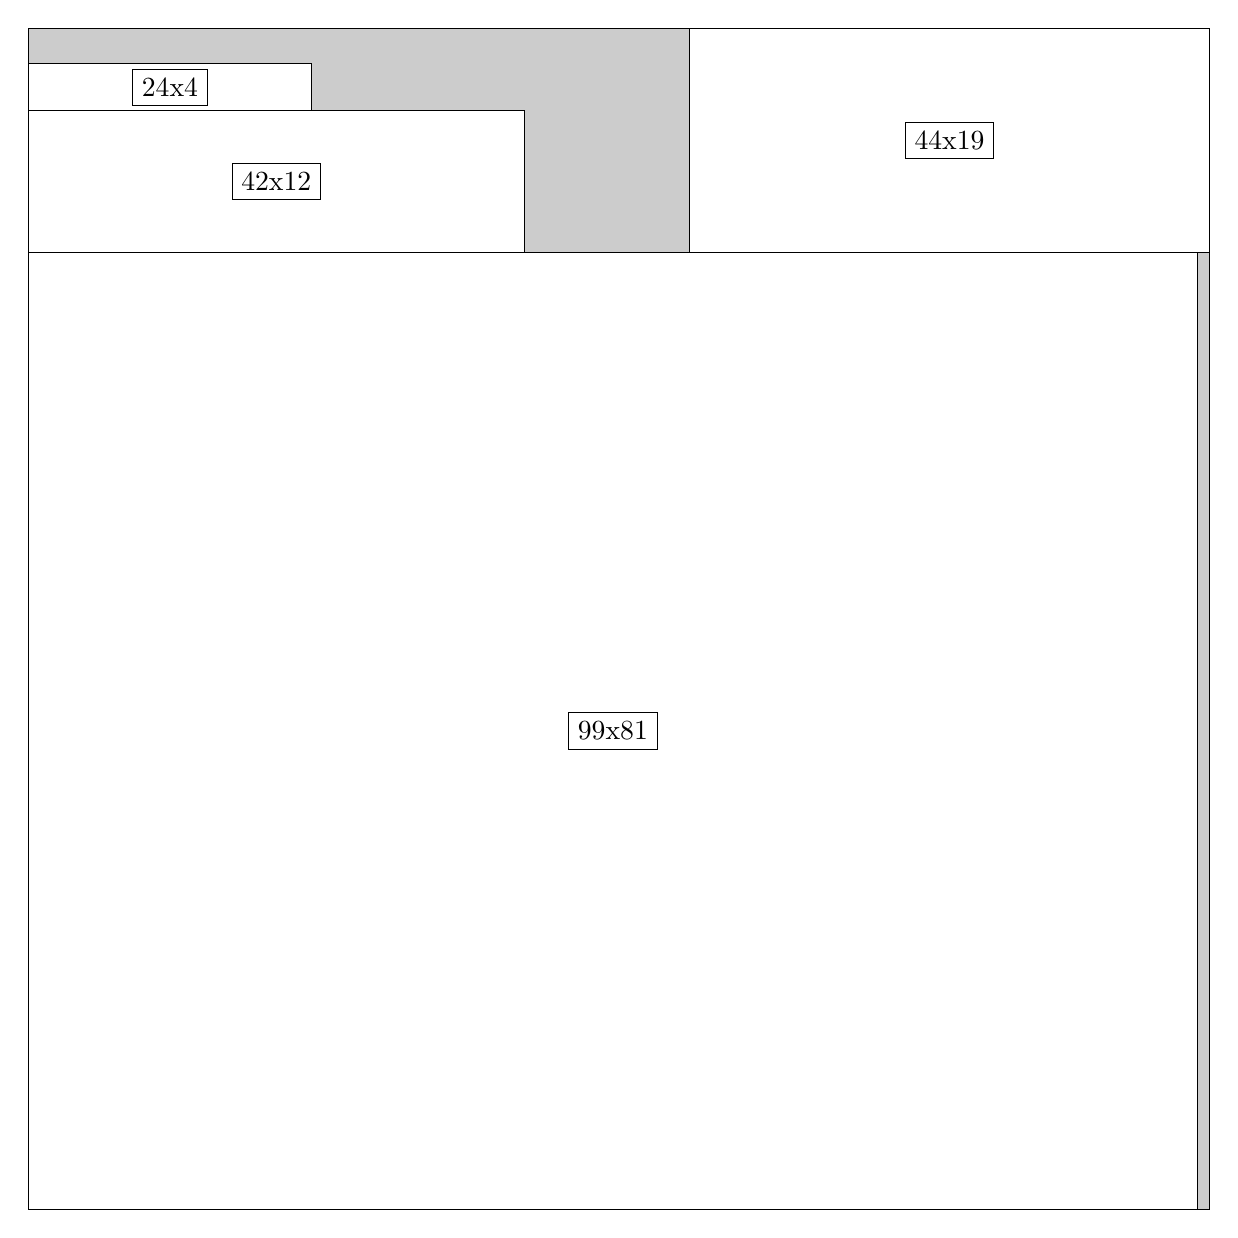
\begin{tikzpicture}[shorten >=1pt,scale=1.0,every node/.style={scale=1.0},->]
\tikzstyle{vertex}=[circle,fill=black!25,minimum size=14pt,inner sep=0pt]
\filldraw[fill=gray!40!white, draw=black] (0,0) rectangle (15.0,15.0);
\foreach \name/\x/\y/\w/\h in {99x81/0.0/0.0/14.85/12.15,44x19/8.4/12.15/6.6/2.85,42x12/0.0/12.15/6.3/1.7999999999999998,24x4/0.0/13.95/3.5999999999999996/0.6}
\filldraw[fill=white!40!white, draw=black] (\x,\y) rectangle node[draw] (\name) {\name} ++(\w,\h);
\end{tikzpicture}


w =99 , h =81 , x =0 , y =0 , v =8019
\par
w =44 , h =19 , x =56 , y =81 , v =836
\par
w =42 , h =12 , x =0 , y =81 , v =504
\par
w =24 , h =4 , x =0 , y =93 , v =96
\par
\newpage


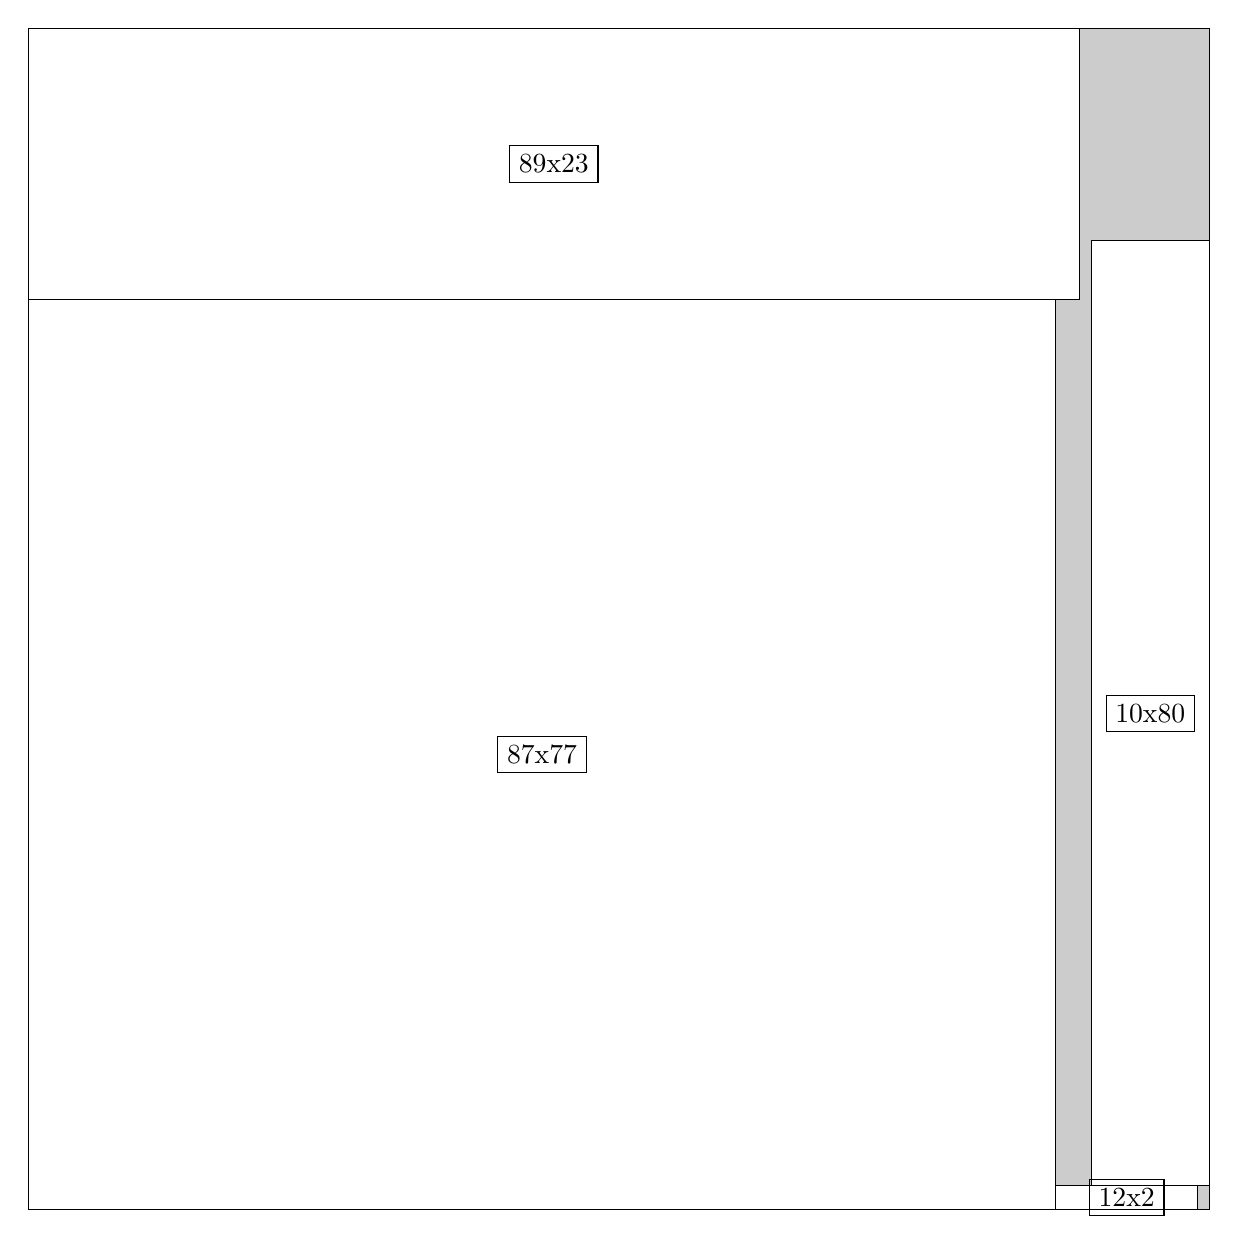
\begin{tikzpicture}[shorten >=1pt,scale=1.0,every node/.style={scale=1.0},->]
\tikzstyle{vertex}=[circle,fill=black!25,minimum size=14pt,inner sep=0pt]
\filldraw[fill=gray!40!white, draw=black] (0,0) rectangle (15.0,15.0);
\foreach \name/\x/\y/\w/\h in {87x77/0.0/0.0/13.049999999999999/11.549999999999999,10x80/13.5/0.3/1.5/12.0,89x23/0.0/11.549999999999999/13.35/3.4499999999999997,12x2/13.049999999999999/0.0/1.7999999999999998/0.3}
\filldraw[fill=white!40!white, draw=black] (\x,\y) rectangle node[draw] (\name) {\name} ++(\w,\h);
\end{tikzpicture}


w =87 , h =77 , x =0 , y =0 , v =6699
\par
w =10 , h =80 , x =90 , y =2 , v =800
\par
w =89 , h =23 , x =0 , y =77 , v =2047
\par
w =12 , h =2 , x =87 , y =0 , v =24
\par
\newpage


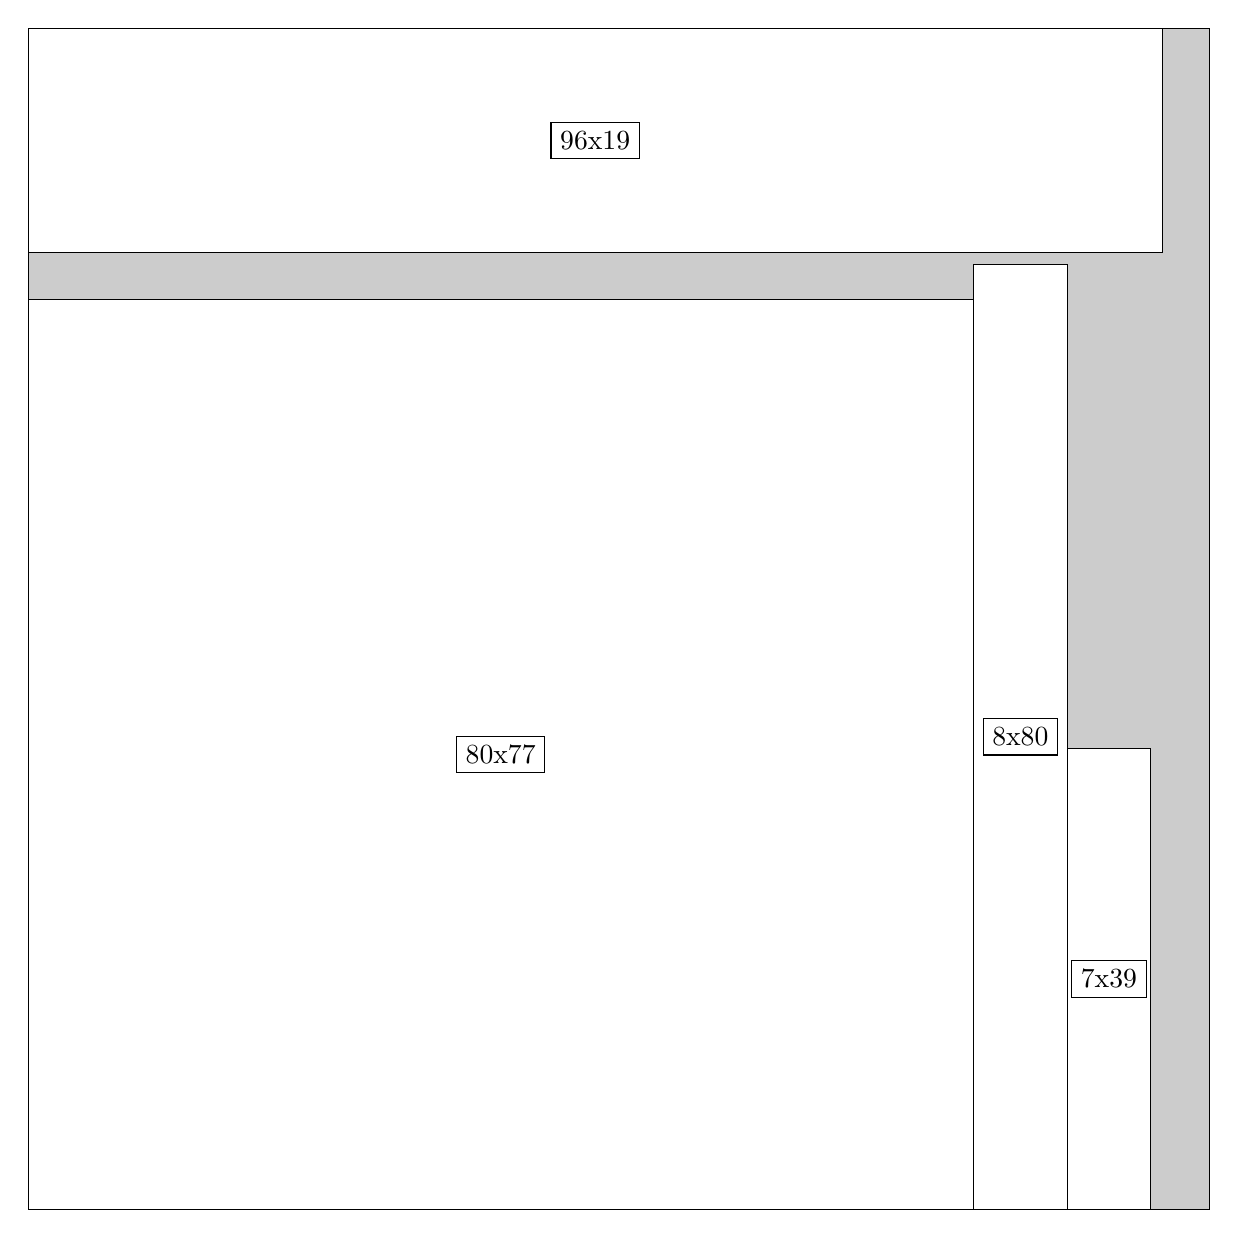
\begin{tikzpicture}[shorten >=1pt,scale=1.0,every node/.style={scale=1.0},->]
\tikzstyle{vertex}=[circle,fill=black!25,minimum size=14pt,inner sep=0pt]
\filldraw[fill=gray!40!white, draw=black] (0,0) rectangle (15.0,15.0);
\foreach \name/\x/\y/\w/\h in {80x77/0.0/0.0/12.0/11.549999999999999,96x19/0.0/12.15/14.399999999999999/2.85,8x80/12.0/0.0/1.2/12.0,7x39/13.2/0.0/1.05/5.85}
\filldraw[fill=white!40!white, draw=black] (\x,\y) rectangle node[draw] (\name) {\name} ++(\w,\h);
\end{tikzpicture}


w =80 , h =77 , x =0 , y =0 , v =6160
\par
w =96 , h =19 , x =0 , y =81 , v =1824
\par
w =8 , h =80 , x =80 , y =0 , v =640
\par
w =7 , h =39 , x =88 , y =0 , v =273
\par
\newpage


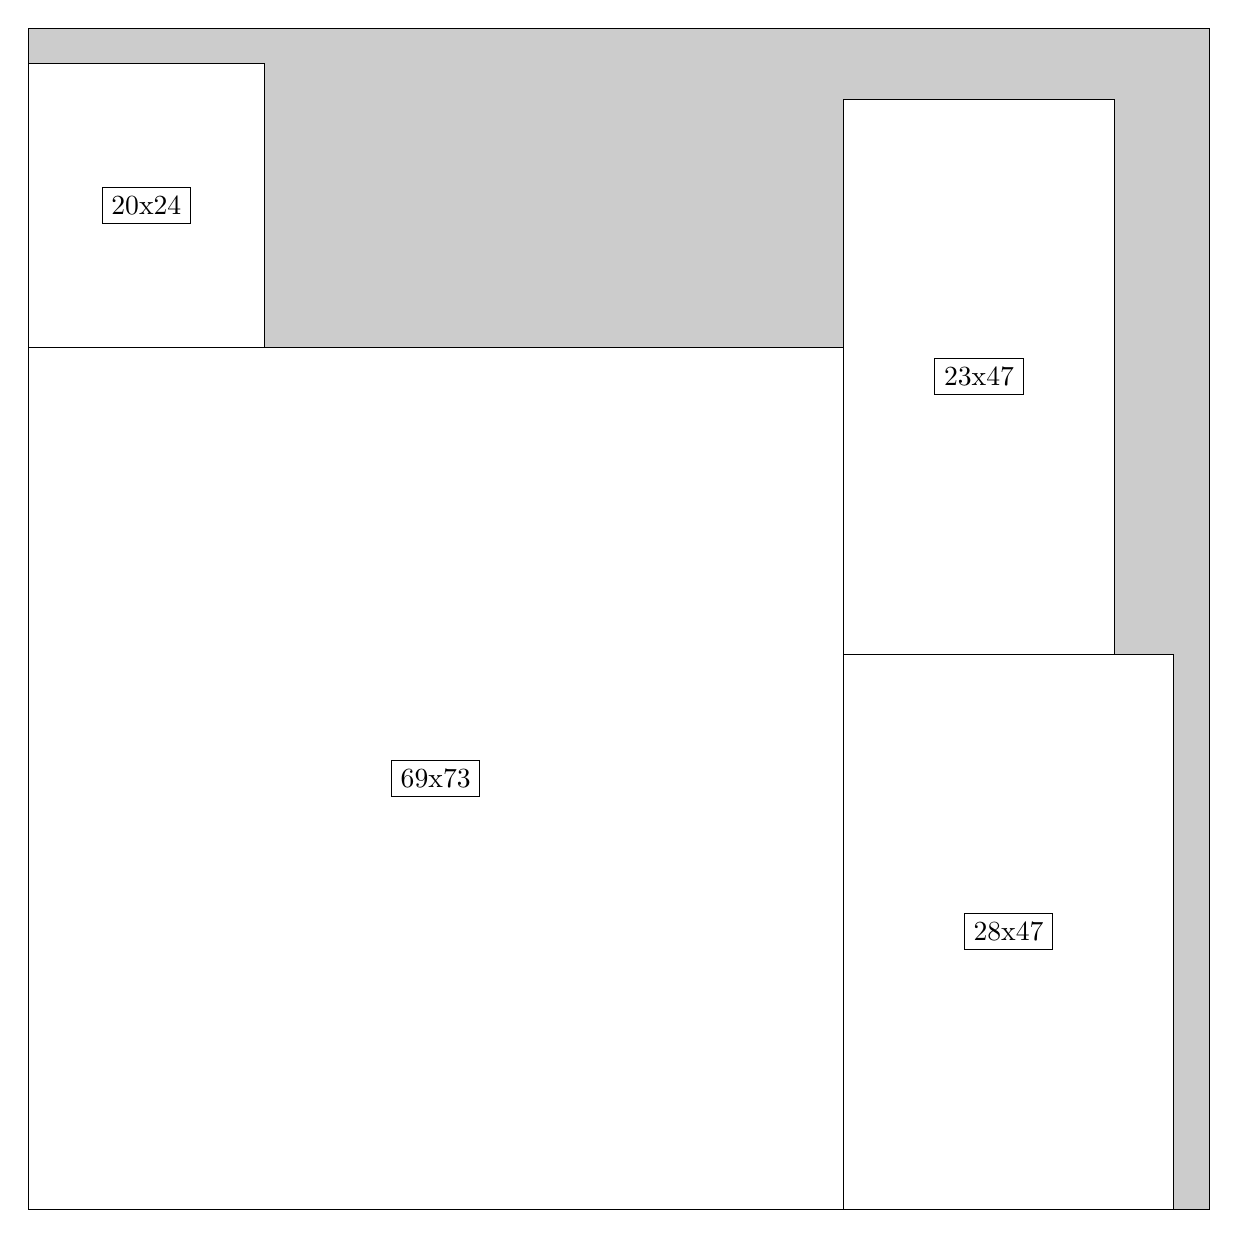
\begin{tikzpicture}[shorten >=1pt,scale=1.0,every node/.style={scale=1.0},->]
\tikzstyle{vertex}=[circle,fill=black!25,minimum size=14pt,inner sep=0pt]
\filldraw[fill=gray!40!white, draw=black] (0,0) rectangle (15.0,15.0);
\foreach \name/\x/\y/\w/\h in {69x73/0.0/0.0/10.35/10.95,28x47/10.35/0.0/4.2/7.05,23x47/10.35/7.05/3.4499999999999997/7.05,20x24/0.0/10.95/3.0/3.5999999999999996}
\filldraw[fill=white!40!white, draw=black] (\x,\y) rectangle node[draw] (\name) {\name} ++(\w,\h);
\end{tikzpicture}


w =69 , h =73 , x =0 , y =0 , v =5037
\par
w =28 , h =47 , x =69 , y =0 , v =1316
\par
w =23 , h =47 , x =69 , y =47 , v =1081
\par
w =20 , h =24 , x =0 , y =73 , v =480
\par
\newpage


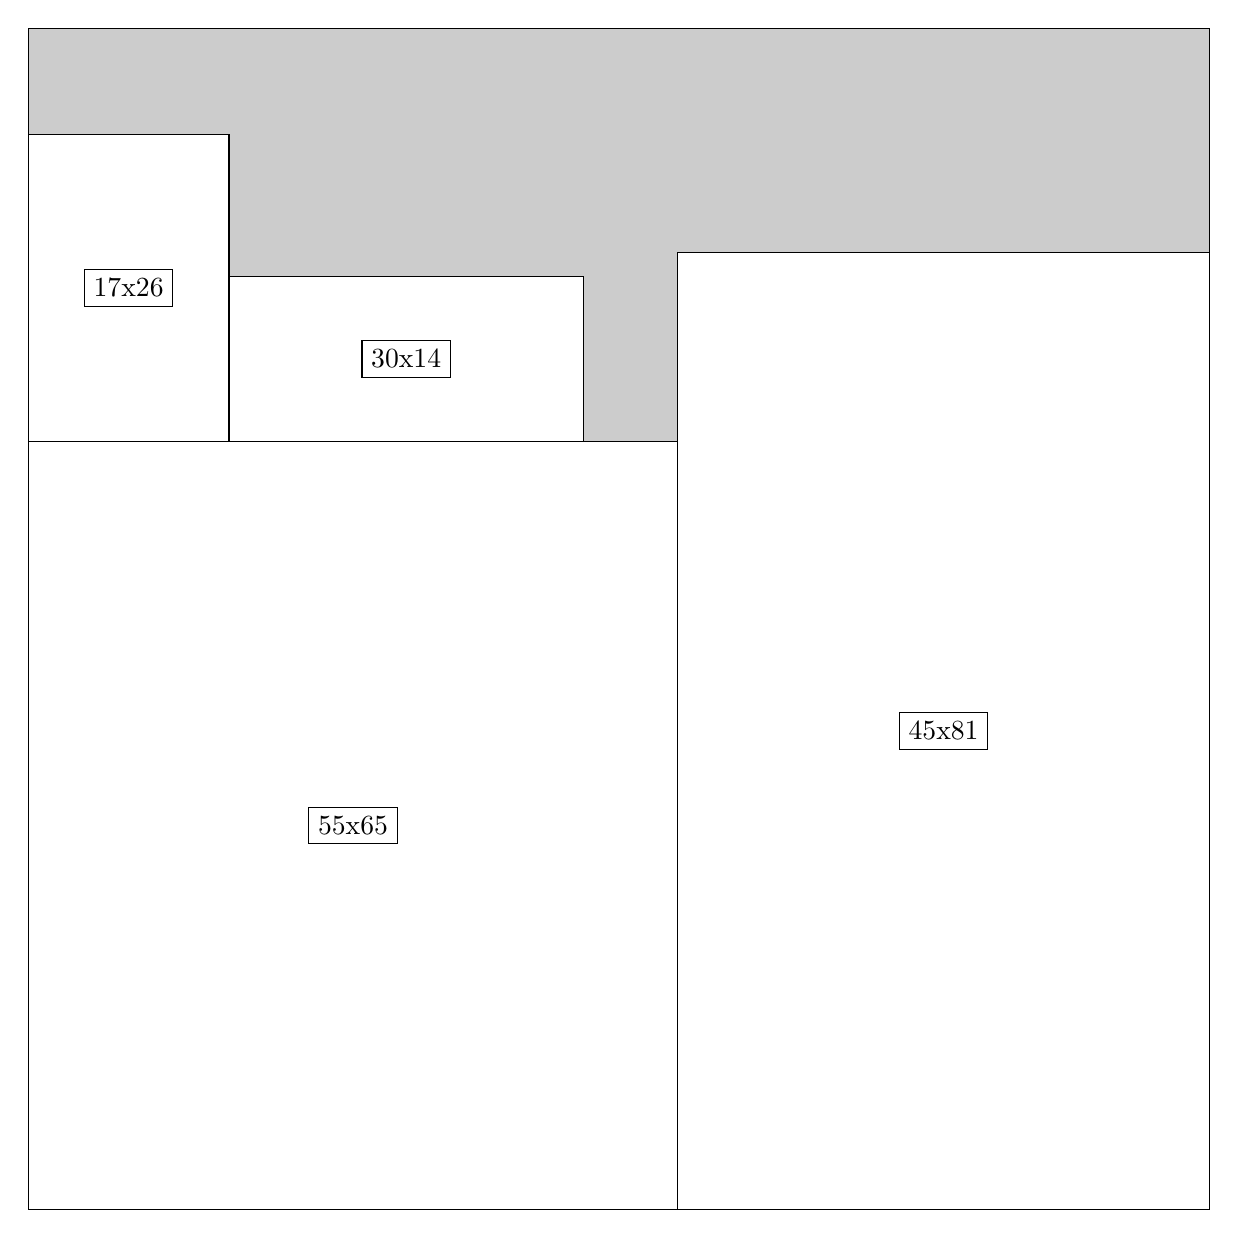
\begin{tikzpicture}[shorten >=1pt,scale=1.0,every node/.style={scale=1.0},->]
\tikzstyle{vertex}=[circle,fill=black!25,minimum size=14pt,inner sep=0pt]
\filldraw[fill=gray!40!white, draw=black] (0,0) rectangle (15.0,15.0);
\foreach \name/\x/\y/\w/\h in {45x81/8.25/0.0/6.75/12.15,55x65/0.0/0.0/8.25/9.75,17x26/0.0/9.75/2.55/3.9,30x14/2.55/9.75/4.5/2.1}
\filldraw[fill=white!40!white, draw=black] (\x,\y) rectangle node[draw] (\name) {\name} ++(\w,\h);
\end{tikzpicture}


w =45 , h =81 , x =55 , y =0 , v =3645
\par
w =55 , h =65 , x =0 , y =0 , v =3575
\par
w =17 , h =26 , x =0 , y =65 , v =442
\par
w =30 , h =14 , x =17 , y =65 , v =420
\par
\newpage


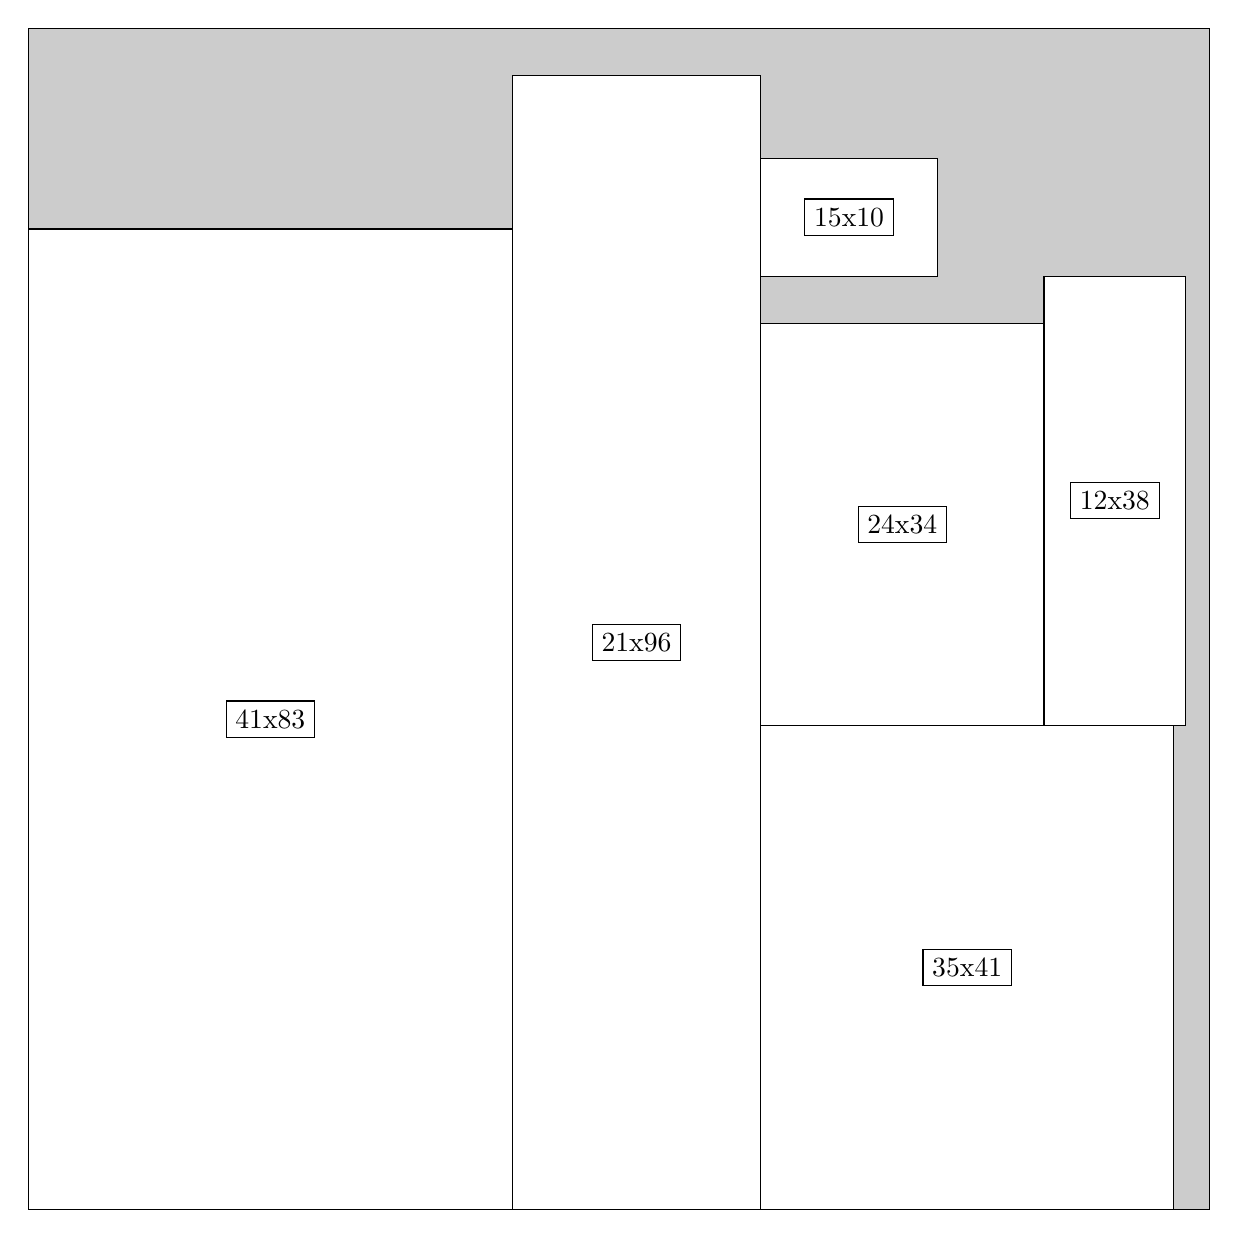
\begin{tikzpicture}[shorten >=1pt,scale=1.0,every node/.style={scale=1.0},->]
\tikzstyle{vertex}=[circle,fill=black!25,minimum size=14pt,inner sep=0pt]
\filldraw[fill=gray!40!white, draw=black] (0,0) rectangle (15.0,15.0);
\foreach \name/\x/\y/\w/\h in {41x83/0.0/0.0/6.1499999999999995/12.45,21x96/6.1499999999999995/0.0/3.15/14.399999999999999,35x41/9.299999999999999/0.0/5.25/6.1499999999999995,12x38/12.9/6.1499999999999995/1.7999999999999998/5.7,15x10/9.299999999999999/11.85/2.25/1.5,24x34/9.299999999999999/6.1499999999999995/3.5999999999999996/5.1}
\filldraw[fill=white!40!white, draw=black] (\x,\y) rectangle node[draw] (\name) {\name} ++(\w,\h);
\end{tikzpicture}


w =41 , h =83 , x =0 , y =0 , v =3403
\par
w =21 , h =96 , x =41 , y =0 , v =2016
\par
w =35 , h =41 , x =62 , y =0 , v =1435
\par
w =12 , h =38 , x =86 , y =41 , v =456
\par
w =15 , h =10 , x =62 , y =79 , v =150
\par
w =24 , h =34 , x =62 , y =41 , v =816
\par
\newpage


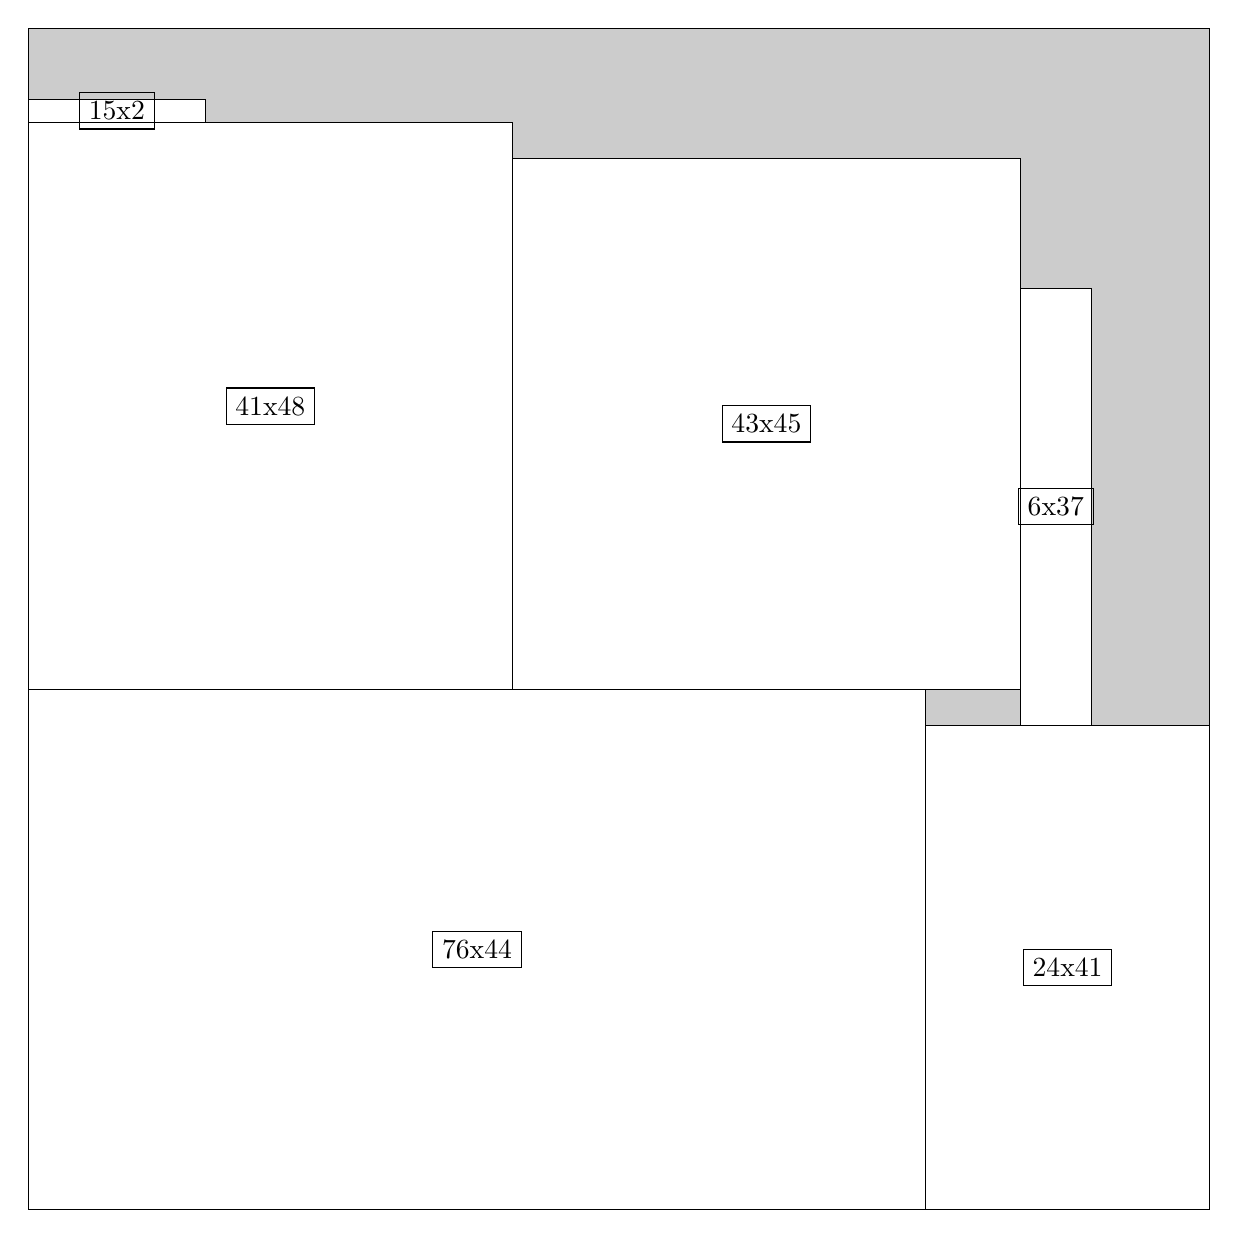
\begin{tikzpicture}[shorten >=1pt,scale=1.0,every node/.style={scale=1.0},->]
\tikzstyle{vertex}=[circle,fill=black!25,minimum size=14pt,inner sep=0pt]
\filldraw[fill=gray!40!white, draw=black] (0,0) rectangle (15.0,15.0);
\foreach \name/\x/\y/\w/\h in {76x44/0.0/0.0/11.4/6.6,41x48/0.0/6.6/6.1499999999999995/7.199999999999999,43x45/6.1499999999999995/6.6/6.45/6.75,24x41/11.4/0.0/3.5999999999999996/6.1499999999999995,15x2/0.0/13.799999999999999/2.25/0.3,6x37/12.6/6.1499999999999995/0.8999999999999999/5.55}
\filldraw[fill=white!40!white, draw=black] (\x,\y) rectangle node[draw] (\name) {\name} ++(\w,\h);
\end{tikzpicture}


w =76 , h =44 , x =0 , y =0 , v =3344
\par
w =41 , h =48 , x =0 , y =44 , v =1968
\par
w =43 , h =45 , x =41 , y =44 , v =1935
\par
w =24 , h =41 , x =76 , y =0 , v =984
\par
w =15 , h =2 , x =0 , y =92 , v =30
\par
w =6 , h =37 , x =84 , y =41 , v =222
\par
\newpage


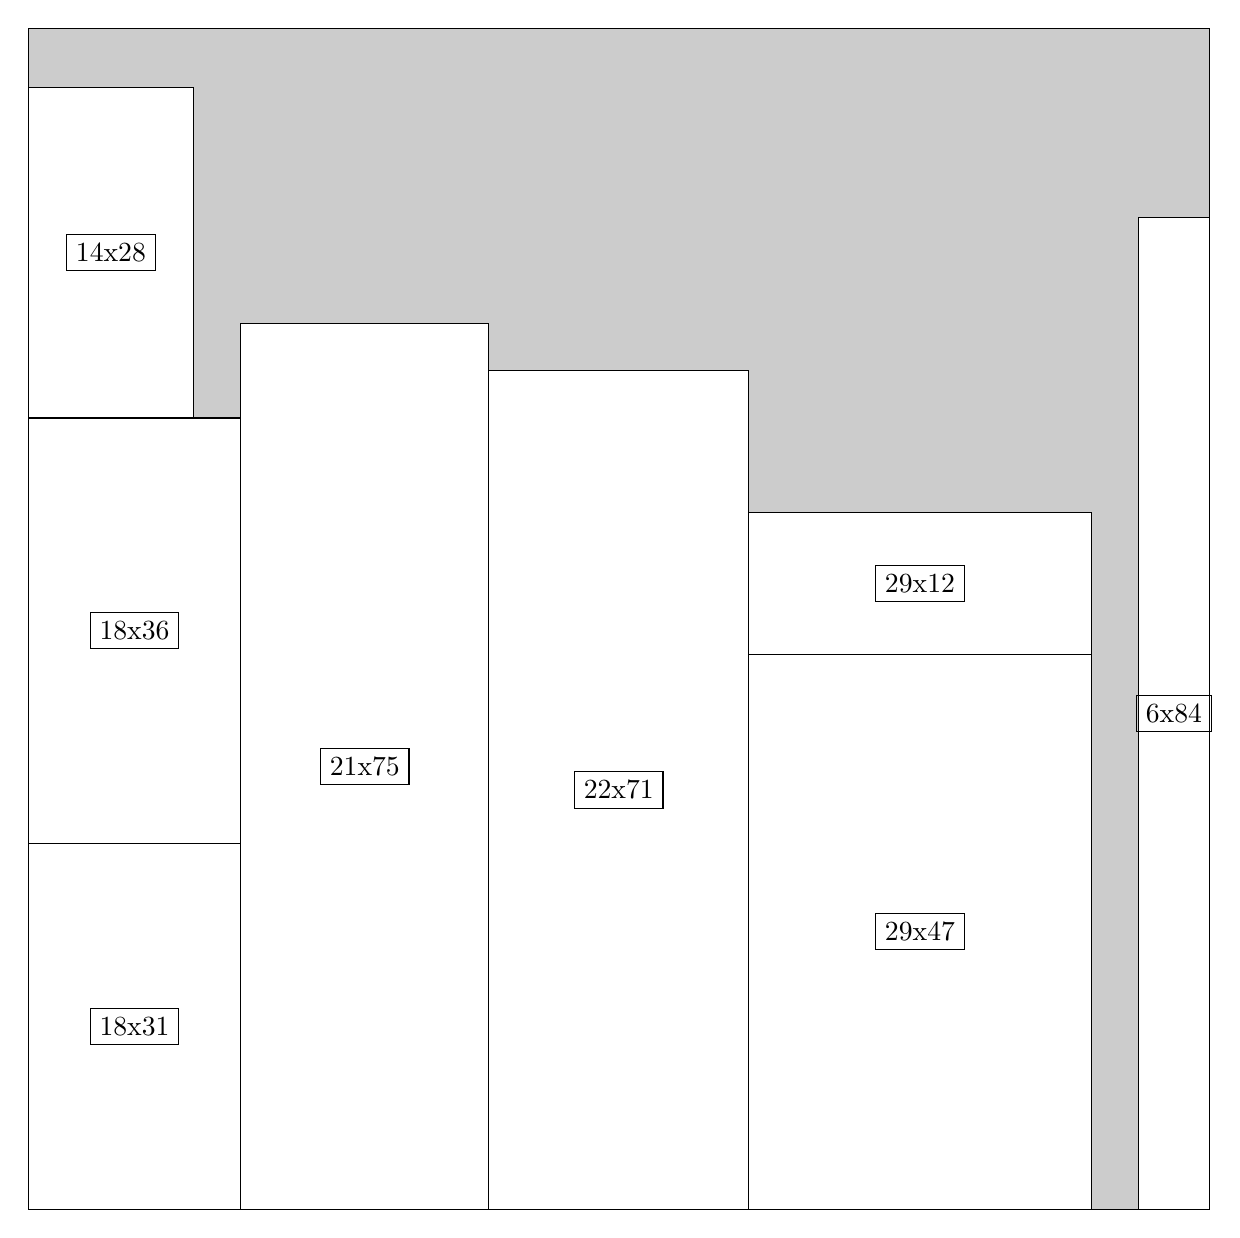
\begin{tikzpicture}[shorten >=1pt,scale=1.0,every node/.style={scale=1.0},->]
\tikzstyle{vertex}=[circle,fill=black!25,minimum size=14pt,inner sep=0pt]
\filldraw[fill=gray!40!white, draw=black] (0,0) rectangle (15.0,15.0);
\foreach \name/\x/\y/\w/\h in {18x31/0.0/0.0/2.6999999999999997/4.6499999999999995,21x75/2.6999999999999997/0.0/3.15/11.25,22x71/5.85/0.0/3.3/10.65,29x47/9.15/0.0/4.35/7.05,18x36/0.0/4.6499999999999995/2.6999999999999997/5.3999999999999995,6x84/14.1/0.0/0.8999999999999999/12.6,14x28/0.0/10.049999999999999/2.1/4.2,29x12/9.15/7.05/4.35/1.7999999999999998}
\filldraw[fill=white!40!white, draw=black] (\x,\y) rectangle node[draw] (\name) {\name} ++(\w,\h);
\end{tikzpicture}


w =18 , h =31 , x =0 , y =0 , v =558
\par
w =21 , h =75 , x =18 , y =0 , v =1575
\par
w =22 , h =71 , x =39 , y =0 , v =1562
\par
w =29 , h =47 , x =61 , y =0 , v =1363
\par
w =18 , h =36 , x =0 , y =31 , v =648
\par
w =6 , h =84 , x =94 , y =0 , v =504
\par
w =14 , h =28 , x =0 , y =67 , v =392
\par
w =29 , h =12 , x =61 , y =47 , v =348
\par
\newpage


\end{document}